%%%%%%%%%%%%%%%%%%%%%%%%%%%%%%%%%%%%%%%%%%%%%%%%%%%%%%%%%%%%%%%%%%%%%%%%%%%%%%%%
\documentclass[paper=a4,fontsize=11pt, hidelinks]{temp} % KOMA-article class

\usepackage{layout} % to visualize layout with \layout
\usepackage[english]{babel}
\usepackage{hyperref} %hyperlinks
\usepackage{fancyhdr}
\usepackage{ifthen} %if then commands
\usepackage{fontawesome} %www.latexdraw.com/wp-content/uploads/2021/01/fontawesome5_2.pdf

% for header/footer
\pagestyle{fancy}
\renewcommand{\headrulewidth}{0pt} %header separation-line width
\renewcommand{\footrulewidth}{0.4pt} %footer separation-line width
\fancyhead[C]{} %header
\cfoot{ %footer
    In compliance with Italian Legislative Decree n.196 dated 30/06/2003, I hereby authorize to use and process my personal details contained in this document.
    \href{https://igor-lirussi.github.io/Curriculum-Vitae/}{Version updated on \today . \underline{Latest Here}} \\
    \thepage %page number
}

%%%%%%%%%%%%%%%%%%%%%%%%%%%%%%%%%%%%%%%%%%%%%%%%%%%%%%%%%%%%%%%%%%%%%%%%%%%%%%
\begin{document}

% Upload your photo and rename it to "photo.png" or "photo.jpg"
\begin{minipage}{0.2\linewidth}
   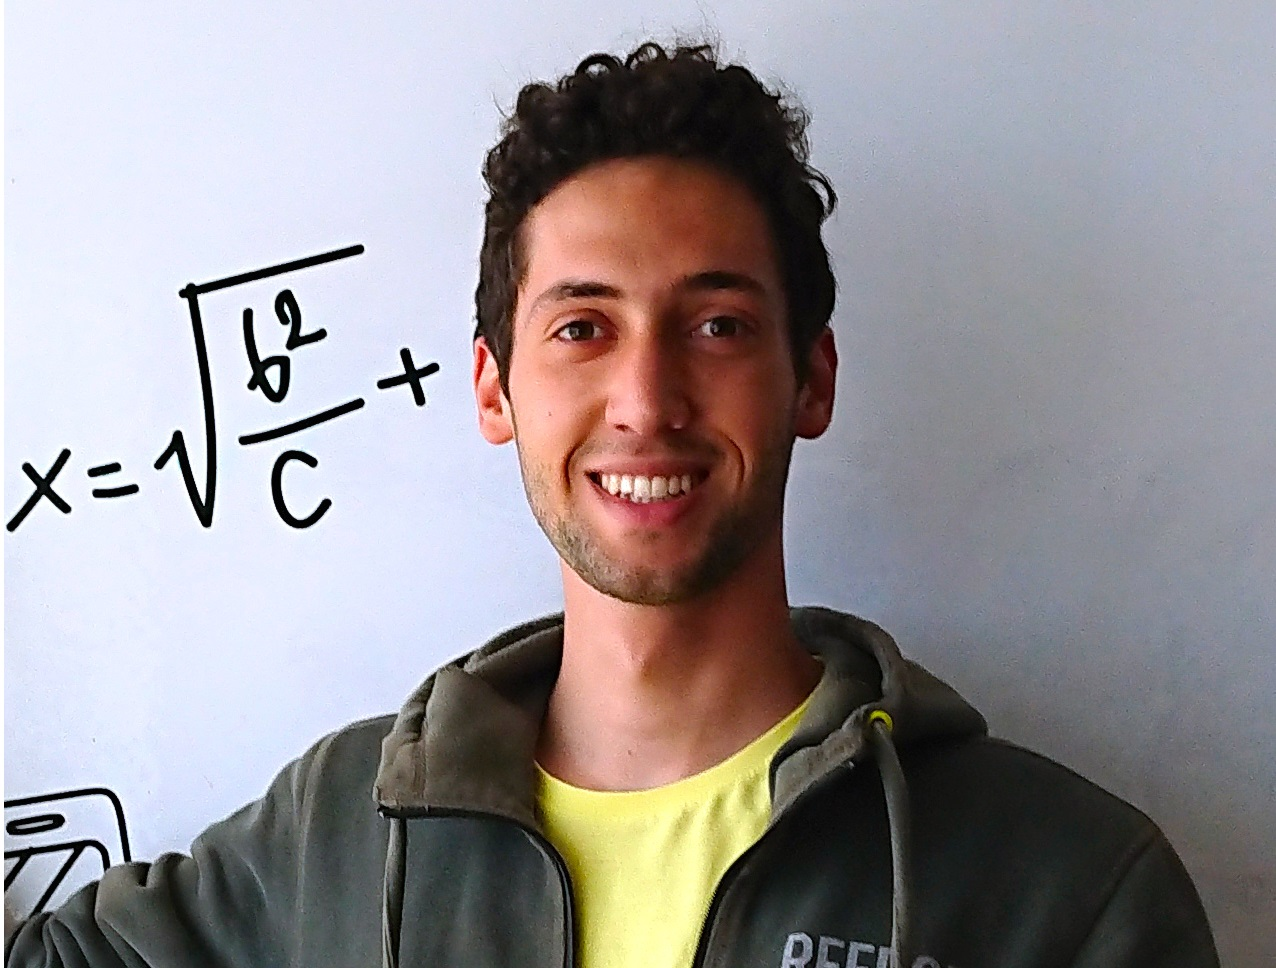
\includegraphics[width=1\textwidth]{photo}
\end{minipage}      
\begin{minipage}{0.75\linewidth}
    \MyName{Igor Lirussi}
    \sepspace
    \noindent
    % info 
    \hfill {\color{headings}Nationality:} Italian | {\color{headings}Birth:} 25/12/1995 | {\color{headings} Gender:} M | {\color{headings} Marital Status:} Single
    
    \hfill {\color{headings}\faEnvelope} \href{mailto:lirussi.igor@gmail.com}{lirussi.igor@gmail.com}
    | {\color{headings}\faPhone}  0039 3317055048 
    
    \hfill \href{https://www.linkedin.com/in/igor-lirussi}{{\color{headings}\faLinkedin\space LinkedIn: }igor-lirussi}| \href{https://igor-lirussi.github.io/ResearchSmall.html}{{\color{headings}\faFolder\space Portfolio: }igor-lirussi.github.io}| \href{https://github.com/igor-lirussi}{{\color{headings}\faGithub\space GitHub:} igor-lirussi}
    
    \hfill {\color{headings}\faMapMarker} via VI Maggio 24, 33030, Forgaria nel Friuli (UD), Italy
 
\end{minipage}


%%%%%%%%%%%%%%%%%%%%%%%%%%%%%%%%%%%%%%%%%%%%%%%%%%%%%%%%%%%%%%%%%%%%%%%%%%%%%%%%
\NewPart{Work Experience}{}
\noindent

\href{https://colors.cmpe.boun.edu.tr}{
\shortEntry{RESEARCHER - COGNITIVE ROBOTICS}
{Oct 2021 - Feb 2024}
{Istanbul (TR) Boğaziçi University: Cognitive Learning and Robotics Laboratory}
{
Enabled industrial and collaborative robots to plan and perform different manipulative actions on objects and assess the results to achieve long-term goals. Particle-simulation physics in VR.
    \ifthenelse{\isShort=0} {%long version
     \begin{itemize}
        \item Cognitive Robotics
        \item Virtual Reality
     \end{itemize}
    }{%short version
     \\Cognitive Robotics and Virtual Reality
    } 
} {IMG/bogazici}
}
\sepspace

\href{https://www.kth.se/is/rpl}{
\shortEntry{RESEARCH ASSISTANT - INTERACTION ROBOTICS}
{Apr 2020 - Sep 2020}
{Stockholm (SE) KTH Royal Institute of Technology: Robotic Perception and Learning Department}
{
Creation of software for natural language interaction with a humanoid robot.
    \ifthenelse{\isShort=0} {%long version
     \begin{itemize}
        \item Human-Robot Interaction
        \item Dialog Engines
     \end{itemize}
    }{%short version
     \\Human-Robot Interaction and Dialog Engines
    } 
} {IMG/kth}
}
\sepspace

\href{https://welcome.isr.tecnico.ulisboa.pt/}{
\shortEntry{RESEARCH SCHOLAR - COMPUTER VISION}
{Sep 2018 - Sep 2019}
{Lisbon (PT) IST Instituto Superior Técnico: I.S.R. Institute for Systems and Robotics - VisLab}
{
Development of software for a mobile robot to navigate indoors and recognize surroundings.
    \ifthenelse{\isShort=0} {%long version
     \begin{itemize}
        \item Object Recognition and Dialog Processing for Human-Robot Interaction
        \item SLAM and Visual Navigation Systems
     \end{itemize}
    }{%short version
     \\Object Recognition, NLP for Human-Robot Interaction, SLAM, and Visual Navigation Systems
    } 
} {IMG/ist}
}

%%%%%%%%%%%%%%%%%%%%%%%%%%%%%%%%%%%%%%%%%%%%%%%%%%%%%%%%%%%%%%%%%%%%%%%%%%%%%%%%
\NewPart{Education}{}
\noindent

\href{https://corsi.unibo.it/2cycle/ComputerScienceEngineering}{
\longEntry{MSc. COMPUTER SCIENCE AND ENGINEERING}
{Sep 2019 - Dec 2023}
{University of Bologna}
{
    \textbf{Thesis: Novel robotic action synthesis with Conditional Neural Movement Primitives.}\\
    \ifthenelse{\isShort=0} {%long version
    Machine Learning, Distributed Systems, Languages, Compilers and Computational Models, Information Systems, Concurrent and Distributed Programming, Programming and Development Paradigms, Web Services and Applications, Smart City and Mobile Technologies, Agile, Continuous Integration and Delivery. 
    }
} 
{IMG/unibo}
}
\sepspace

\href{https://dsv.su.se/en/}{
\longEntry{INTERNATIONAL STUDENT MSc.}
{Jan 2020 - Jul 2020}
{Stockholm University}
{Decision Making and Business Intelligence, Network Security, Cyber Forensics}
{IMG/stockholmuni}
}
\sepspace

\href{https://ciencias.ulisboa.pt/en}{
\longEntry{INTERNATIONAL STUDENT BSc.}
{Sep 2018 - Sep 2019}
{Lisbon University}
{Artificial Intelligence, Operational Research} 
{IMG/ulisboa}
}
\sepspace

\href{https://corsi.unibo.it/1cycle/ComputerScienceEngineering}{
\longEntry{BSc. COMPUTER SCIENCE AND ENGINEERING}
{Sep 2014 - Sep 2019}
{University of Bologna}
{
    \textbf{Thesis: Framework for navigation and Human-Robot interaction with humanoid robots.}\\
    \ifthenelse{\isShort=0} {%long version
    Software Engineering, Embedded Systems and IoT, Automatic Controls, Mobile App Programming, Operating Systems, Object-Oriented Programming, Network Programming, Telecommunications Networks, Law for Information Technology, Fundamentals of Image Processing, Databases, Algorithms and Data Structures, Computer Architecture, C Programming
    }
} 
{IMG/unibo}
}

%%%%%%%%%%%%%%%%%%%%%%%%%%%%%%%%%%%%%%%%%%%%%%%%%%%%%%%%%%%%%%%%%%%%%%%%%%%%%%%%
\NewPart{ Technical Skills \& Software }{}
\begin{minipage}[t]{0.67\textwidth} 
\ifthenelse{\isShort=0} {%long version
    \begin{itemize}
    \item \href{https://github.com/igor-lirussi}{Mastery of programming paradigms (imperative, OOP, functional, logic, concurrent) and languages (Python, Java, Scala, Bash scripting, C, C++, C\#, HTML-CSS, PHP, Javascript, Assembly, Prolog, SQL).}
    \item Advanced knowledge of Digital Image Processing/Image Elaboration/Template Matching and Computer Vision algorithms.
    \item Proficient understanding of software for automation, robotics internal dynamics of micro-controllers, IoT, embedded systems, and operation of sensors and mechanical actuators.
    \item Competent knowledge of high-performance and data-intensive computing, Machine Learning, and BI.
    \item Advanced skills in video/photo editing programs, video making, GUI and graphics design.
    \end{itemize}
}{%short version
    \begin{tabular}[t]{ l }
    Programming paradigms: imperative/OO/functional/logic/concurrent.\\
    Languages: C, C++, C\#, Java, Scala, Bash scripting, Python.\\
    Advanced knowledge of embedded systems and automation, \\
    Image processing algorithms, machine learning, video/photo editing.\\
    \end{tabular}
}
\end{minipage}
%
\begin{minipage}[t]{0.32\textwidth} 
\begin{tabular}[t]{ r l }
\software{IMG/software/git}  & Git/GitHub Actions/Projects\\
\software{IMG/software/opencv}  & OpenCV\\
\software{IMG/software/ros}  & ROS\\
\software{IMG/software/pytorch}  & PyTorch
\ifthenelse{\isShort=0} {%long version
    \\
    \software{IMG/software/unity} & Unity \\
    \software{IMG/software/esp} & Esp32/Arduino/Raspberry\\
    \software{IMG/software/latex}  & LaTeX Writing \\
    \software{IMG/software/office} & Office Suite \\
    \software{IMG/software/premiere}  & Adobe Premiere Pro\\
}{}
\end{tabular}
\end{minipage}

%%%%%%%%%%%%%%%%%%%%%%%%%%%%%%%%%%%%%%%%%%%%%%%%%%%%%%%%%%%%%%%%%%%%%%%%%%%%%%%%
\NewPart{Languages \& Interests}{}
\hspace{3mm} %space on the sides
\begin{minipage}[t]{0.32\textwidth} 
%Languages (ISO 639-1)
\begin{tabular}[t]{ l c l }
\flag{IMG/flag/it} & IT & Native Speaker \\
\flag{IMG/flag/gb} & EN & \href{https://github.com/igor-lirussi/Curriculum-Vitae/raw/main/Certificates/IELTS_LIRUSSI.pdf}{Full Proficiency}\\
\flag{IMG/flag/pt} & PT & \href{https://github.com/igor-lirussi/Curriculum-Vitae/raw/main/Certificates/cert_PT_LIRUSSI.pdf}{Conversational}\\
\flag{IMG/flag/sv} & SV & \href{https://github.com/igor-lirussi/Curriculum-Vitae/raw/main/Certificates/cert_SE_LIRUSSI.pdf}{Basic level}\\
\flag{IMG/flag/tr} & TR & \href{https://github.com/igor-lirussi/Curriculum-Vitae/raw/main/Certificates/cert_TR_LIRUSSI.pdf}{Basic level}\\
%\flag{IMG/flag/de} & DE & A2 & \href{https://github.com/igor-lirussi/Curriculum-Vitae/raw/main/Certificates/cert_DE_LIRUSSI.pdf}{Basic level}\\
\end{tabular}
\end{minipage}
%
\begin{minipage}[t]{0.65\textwidth} 
\begin{tabular}[t]{ l }
\href{https://site.unibo.it/startupdayunibo/en/}{Winner "The 30 new emerging ideas of 2021" - Startup Day Unibo}\\
Theoretical and Practical course of First Aid for companies\\
Cooking and DIY Enthusiast\\
Sport and Videomaking Passionate\\
Food Aid Program Volunteer - Blood Donor\\
\end{tabular}
\end{minipage}


%%% References

\end{document}
